\subsection*{Background}

Clinical trials are considered the gold standard for evaluated of medical intervention [cite].

Principles of beneficence, etc.. (check ICH guidelines) mean that all interventions must in principle be evaluated for both efficacy and safety and further these benefits must outweigh the risks [cite]. Traditionally the efficacy and safety effects are evaluated using a series of trials with four sequential phases. Phase I are first-in-human trials designs usually performed on a small number of healthy participants to determine dosing (and other PK/PD?). Phase II trials are often first to test intervention in patients with the disease of interest and are used to determine efficacy and make go/no-go decision about whether to continue drug development. Phase III trials confirm the efficacy found in early studies and gather more information about adverse events. These studies are usually the pivotal studies required by regulatory agencies to approve a drug for marketing. Finally, Phase IV studies are ongoing surveillance ... [cite]

Usually the effect of treatment on efficacy and safety outcomes are explored with separate models for each type of outcome

Further, many studies include several outcomes (endpoints) of interest represent the effects of the intervention on a multiple (pathologies/disease processes?) and interest may

Same with multiple types of adverse event

For all these situations, modeling outcomes jointly uses data more efficiently [CITE] and provides a better characterization of the intervention across multiple domains[word choice?] simultaneously

(Can occur at multiple phases - phase I/II dosing toxicity/efficacy, phase III benefit-risk , phase IV? adverse risk assessment)

Several strategies have been proposed for such joint models including blah, blah [cite]. In this report I will focus on use of copulas for joint  models\cite{costa_bayesian_2018}. 
 
\subsection*{Copulas} %Brief lit review of field

In the usual case, each outcome is modeled by a univariate function of treatment and and other covariates

A copula is a mathematical function that combines univariate distributions to create a multivariate distribution. Importantly, Sklar's Theorem[cite] guarantees that a proper multivariate distribution function can be constructed by combining any univariate distribution functions (any?? check discrete) and a copula 

this is an example of a citation \cite{nelsen_introduction_2006}.

A distinct advantage of the copula approach is the ability to "couple" arbitrary univariate models, thereby allowing modeling of the marginal univariate outcomes to be separated from modeling of the copula, which contains information about the correlation (more general term) between the outcomes

Further details on copulas and copula regression are presented below 

this is another citation \cite{joe_dependence_2015}

We can also include a picture as seen in figure \ref{Fi:gumbel_cop}. it's a placeholder for now

\begin{figure}
\begin{center}
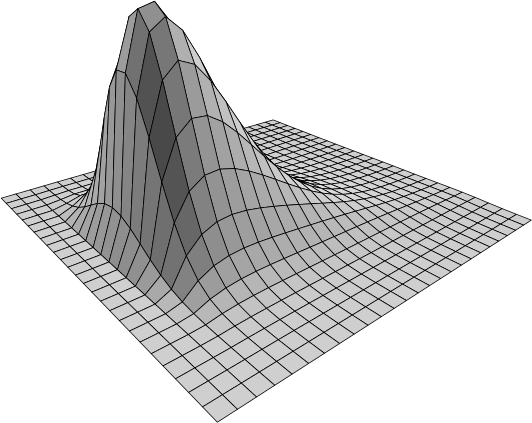
\includegraphics[scale=.4]{fig/gumbel_cop}
\caption{Gumbel copula}
\label{Fi:gumbel_cop}
\end{center}
\end{figure}

\subsection*{Inference}

Inference on the resulting multivariate distribution function can be used to determine how the outcomes are correlated and can be performed under several paradigms 

-Frequentist

-Bayesian

Principled method of combining prior beliefs concerning parameters with additional data

\begin{gather}
p(\theta|y)=\frac{p(y|\theta)p(\theta)}{\int p(y|\theta)p(\theta)\,d\theta}
\end{gather}

In context of clinical trials - include elicited clinical expertise, previous (historical) studies

Inference based on posterior probabilities more interpretable

Adaptive designs??

-Likelihood??




